\chapter{Einleitung}


Durch den immer weiter fortschreitenden Umstieg auf erneuerbare Energien werden gute Möglichkeiten zur Speicherung der gewonnenen Energie zunehmend wichtiger -- dies resultiert in einem entsprechend hohen Forschungsinteresse. Ein Vorschlag für eine neue Technologie ist die Nutzung von ionischen Flüssigkeiten. Um aber am Ende effiziente Produkte herstellen zu können, müssen die physikalischen Vorgänge in diesen Substanzen auf mikroskopischer Ebene verstanden sein. Dies betrifft insbesondere die Struktur und Dynamik von Molekülen und Atomen. 

Dafür kann die magnetische Kernspinresonanz (kurz NMR vom engl. „magnetic nuclear resonance“) eine hilfreiche Methode sein, ist sie doch beispielsweise für die Auflösung von Strukturen ein allgegenwärtig verwendetes Werkzeug in der Chemie. Aber auch die Möglichkeit, die Untersuchung auf ein bestimmtes Isotop zu beschränken, macht es möglich, den Einfluss der Dynamik von verschiedenen Komponenten eines Moleküls separat zu untersuchen.

In dieser Arbeit wurde Calciumrubidiumnitrat, $[\text{Ca}(\text{NO}_\text{3})_\text{2}]_\text{2}[\text{RbNO}_\text{3}]_\text{3}$ kurz CRN, mit $^\text{87}$Rb-NMR untersucht. Dabei handelt es sich um ein Nitratsalz, welches bei entsprechend schnellem Abkühlen ein Glas, also einen amorphen Feststoff, bildet. Dabei „friert“ die Bewegung der Atome oder Moleküle ein, ehe sie einen Gleichgewichtszustand erreichen können. Dies geschieht in der Nähe der Glasübergangstemperatur, welche bei CRN bei $T_g = \SI{333}{\kelvin}$ liegt. Aber auch unterhalb der Glasübergangstemperatur kann es noch -- lokale -- Prozesse geben, welche zu einer Relaxation beitragen. Diese Prozesse werden Betaprozesse genannt -- im Gegensatz zu den Bewegungen oberhalb der Glasübergangstemperatur, welche als Alphaprozess bezeichnet werden und bei dieser einfrieren. Dementsprechend ist in Abbildung \ref{fig:einl:zuernpaper} zu erkennen, dass die Zeitkonstante des Alphaprozesses immer stärker ansteigt, je näher sie der Glasübergangstemperatur bei $\SI{333}{\kelvin}$ kommt.

Vorhergegangene Untersuchungen von CRN umfassen unter anderem die Untersuchungen von C. Zürn, welcher sich ebenfalls mit der $^\text{87}$Rb-NMR beschäftigt hat \cite{zuern_paper} und auf dessen Ergebnissen diese Arbeit teilweise aufbaut.
\begin{figure}
	\begin{center}
		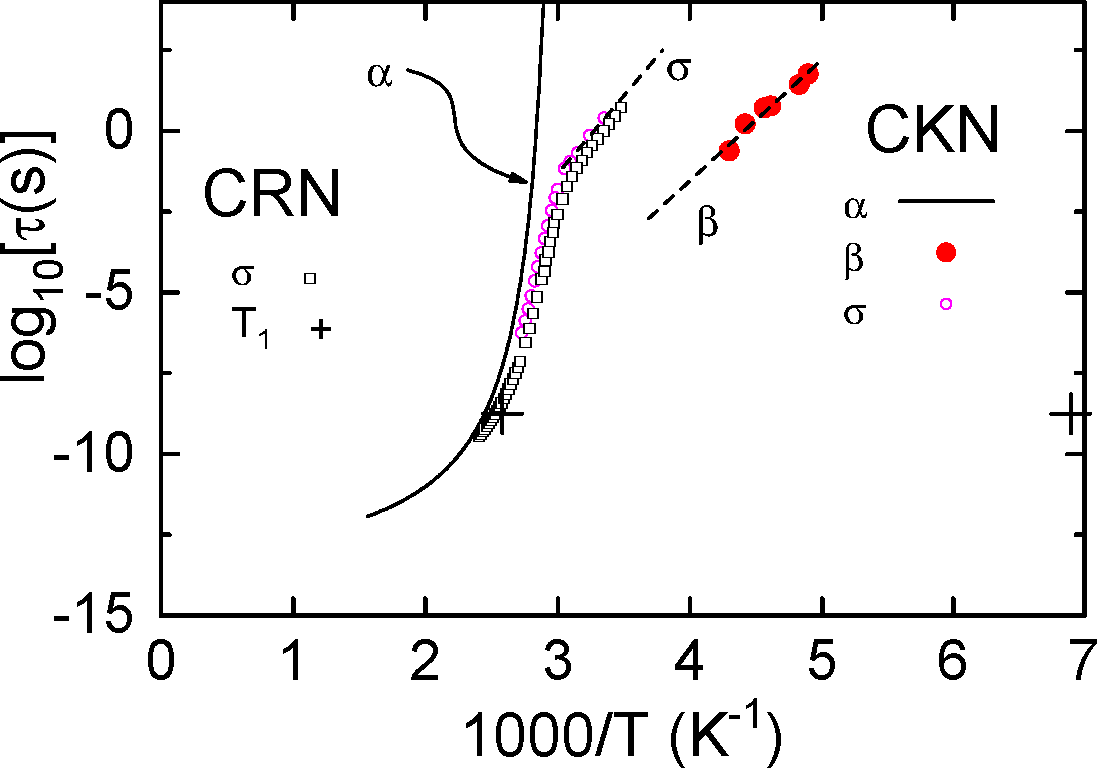
\includegraphics[width=.7\textwidth]{graphics/zuern/Plot1_b2.pdf}
	\end{center}
	\caption{Bearbeitete Relaxationskarte aus \cite{zuern_paper}, dargestellt in einem Arrhenius-Diagramm (logarithmierte Zeitkonstanten aufgetragen gegen die inverse Temperatur). Gezeigt sind ermittelte Zeitkonstanten aus Untersuchungen an CRN und CKN. Hierbei sind für diese Arbeit insbesondere der Betaprozess, dargestellt in rot, interessant. Die Daten hierzu stammen aus \cite{johari_beta}.} \label{fig:einl:zuernpaper}
\end{figure}

Eine Graph aus diesem Paper ist in Abbildung \ref{fig:einl:zuernpaper} zu sehen. Hier sind in CKN, kurz für Calciumkaliumnitrat, entdeckte Hinweise auf einen Betaprozess, dargestellt in rot, hervorzuheben. Die Stoffe CKN und CRN ähneln sich sehr. Bis auf das gegen ein Rubidium-Atom ausgetauschte Kalium-Atom, welches der gleichen Hauptgruppe entstammt, teilen sie die gleiche Struktur, Glasübergangstemperatur und weitere Eigenschaften \cite{PIMENOV199793}. So ist beispielsweise auch die Übereinstimmung von Leitfähigkeitsdaten $\sigma$ zwischen CRN und CKN zu erkennen. Daher ist es nachvollziehbar, für CRN und CKN ähnliche Zeitkonstanten eines Betaprozesses zu erwarten.

Die gestrichelte Linie in Abbildung \ref{fig:einl:zuernpaper} durch die Punkte des Betaprozesses zeigt die lineare Fortsetzung dieser Punkte im Arrhenius-Diagramm an. Wenn dieser Trend standhält, sollten bei Temperaturen in Bereichen kurz unter oder bei der Glasübergangstemperatur von $T_g = \SI{333}{K}$ Zeitkonstanten im hohen Mikrosekunden-Bereich zu erwarten sein. Zeitkonstanten dieser Größenordnungen lassen sich mit Methoden der NMR -- zum Beispiel der hier verwendeten Untersuchung von stimulierten Echos oder der Analyse von Linienformen von pulslängenabhängigen Spektren -- gut untersuchen.

Stimulierte Echos werden vor allen an Kernen, welche nicht-selektiv anregbar sind -- dies ist bei Kernen mit einem schmalen NMR-Spektrum von weniger als ungefähr $\SI{100}{MHz}$ Breite der Fall, durchgeführt. In der Arbeit \cite{joachim_master} wurde jedoch -- an CRN -- gezeigt, dass dies auch für $^\text{87}$Rb, welches nur selektiv anregbar ist, möglich ist.

Während der im Rahmen dieser Arbeit durchgeführten Messungen wurde entdeckt, dass die Halbwertsbreite von CRN-Spektren zu höheren Temperaturen erst abnimmt -- was aufgrund der ansteigenden Bewegungsverschmälerung, dem Herausmitteln von Effekten aufgrund einer höheren Bewegung der Atome und Moleküle, zu höheren Temperaturen zu erwarten ist --, aber bei Temperaturen ab $\SI{375}{K}$ wieder zunimmt. Dies widerspricht der naiven Erwartung, dass die Halbwertsbreite zu steigenden Temperaturen in diesem Fall lediglich abnehmen sollte. Um die Gründe dieses Phänomen zu klären, wurden Spektren simuliert und ein Vergleich mit der Theorie der Quadrupol-Wechselwirkung zweiter Ordnung, welche hier entscheidende Einflüsse hat, durchgeführt.

Zunächst sollen in Kapitel \ref{chapter:theo} die theoretischen Grundlagen der NMR erläutert werden und eine Einführung in die Relaxation der Quadrupol-Wechselwirkung zweiter Ordnung gegeben werden. Kapitel \ref{chapter:simulation} beschreibt die für die Simulation verwendete Software mit zugehörigem Bewegungsmodell. Außerdem wird ein weiteres Bewegungsmodell vorgestellt, das in der Zukunft facettiertere Untersuchungen ermöglichen könnte. In Kapitel \ref{chapter:exp_details} werden die verwendeten Apparaturen und Proben beschrieben, ehe in Kapitel \ref{chapter:experiment} die aufgenommenen Daten zunächst gezeigt, und dann ausgewertet und analysiert werden. Eine Zusammenfassung der Ergebnisse und ein Ausblick auf mögliche zukünftige Untersuchungen bilden den Abschluss der Arbeit.
